\documentclass[aps,pra,onecolumn,notitlepage,superscriptaddress]{revtex4-1}

%\input{myQcircuit}
\usepackage{graphicx,color}% Include figure files
\usepackage{dcolumn}% Align table columns on decimal point
\usepackage{bm}% bold math
\usepackage{amsmath,amssymb,mathrsfs}
\usepackage{url}
\usepackage{hyperref}
\usepackage{framed}
\usepackage{algorithm}
\usepackage{algpseudocode}
\usepackage{wrapfig}
\usepackage{mathtools}
\usepackage{listings}


\newcommand{\N}{\mathbb{N}}
\newcommand{\Z}{\mathbb{Z}}
\newcommand{\R}{\mathbb{R}}
\newcommand{\C}{\mathbb{C}}
\newcommand{\Q}{\mathbb{Q}}


%  Sets
\newcommand{\set}[1]{\mathsf{#1}}
\newcommand{\grp}[1]{\mathsf{#1}}
\newcommand{\spc}[1]{\mathcal{#1}}

% Integrals

\def\d{{\rm d}}

% Linear structures
\newcommand{\Span}{{\mathsf{Span}}}
\newcommand{\Lin}{\mathsf{Lin}}
\newcommand{\rank}{\mathsf{rank}}

\def\>{\rangle}
\def\<{\langle}
\def\kk{\>\!\>}
\def\bb{\<\!\<}
\def\l{\leftarrow}
\def\r{\rightarrow}
\def\u{\underline}
\def\y{\vdash}
\def\ys{\vdash^*}
\newcommand{\st}[1]{\mathbf{#1}}
\newcommand{\bs}[1]{\boldsymbol{#1}}

% Linear maps
\newcommand{\map}[1]{\mathcal{#1}}
\newcommand{\Tr}{\operatorname{Tr}}
\newcommand{\diag}{\mathsf{diag}}

% languages
\newcommand{\reg}{\mathsf{reg}}
\newcommand{\Lan}{\mathsf{L}}


%  Operational notions
\newcommand{\op}[1]{\operatorname{#1}}

\newcommand{\St}{{\mathsf{St}}}
\newcommand{\Eff}{{\mathsf{Eff}}}
\newcommand{\Pur}{{\mathsf{Pur}}}
\newcommand{\Transf}{{\mathsf{Transf}}}
\newcommand{\Chan}{{\mathsf{Chan}}}


%   By Mo
\newcommand{\arccot}{\mathrm{arccot}\,}

%  Miscellanea
\newcommand\myuparrow{\mathord{\uparrow}}
\newcommand\mydownarrow{\mathord{\downarrow}}
\newcommand\h{{\scriptstyle \frac 12}}

% Environments
\newtheorem{theo}{Theorem}
\newtheorem{ax}{Axiom}
\newtheorem{lemma}{Lemma}
\newtheorem{prop}{Proposition}
\newtheorem{cor}{Corollary}
\newtheorem{defi}{Definition}


\newtheorem{rem}{Remark}
\newtheorem{ex}{Exercise}
\newtheorem{proper}{Property}
\newtheorem{exa}{Example}

\def\Proof{{\bf Proof.~}}
\def\qed{$\blacksquare$ \newline}

\begin{document}
	\preprint{APS/123-QED}
    \title{Elements of Computation Theory}
    \author{}
    \maketitle
    % \tableofcontents
    % \newpage
    
    \section{ Alphabet and languages}
    \begin{defi}
        Alphabet and languages
        \begin{itemize}
            \item alphabet $\Sigma$: a finite set of symbols
            \item string: a finite sequence of symbols. Empty string is denoted $e$.
            \item the set of strings over $\Sigma$: $\Sigma^*$
            \item language: any subset of $\Sigma^*$
        \end{itemize}
    \end{defi}

    \begin{defi}
        Operations on languages
        \begin{itemize}
            \item concatenation: $L_1L_2 = \{ w \in \Sigma^* : w = xy, \ x \in L_1,\ y \in L_2 \}$
            \item complement: $\overline{L} = \Sigma^* - L$
            \item Kleene star: $L^* = \{ w \in \Sigma^* : w = w_1\cdots w_k, \ k \geq 0,\ w_1, \cdots, w_k \in L \}$
            \item If $L \neq \emptyset$, define $L^+ = LL^* = \{ w \in \Sigma^* : w = w_1\cdots w_k, \ k \geq 1,\ w_1, \cdots, w_k \in L \}$
        \end{itemize}
    \end{defi}

    \begin{rem}
        $\emptyset$ and $\{ e \}$ are different languages. The former has no strings, and the latter has only the empty string $e$. A special case of Kleene star: $\emptyset^* = \{ e \}$. 
    \end{rem}

    \begin{theo}
        The set of strings over a finite (even countably infinite) alphabet $\Sigma$ is countably infinite. 
    \end{theo}
    The members of $\Sigma^*$ can then be enumerated in the following way.
    \begin{enumerate}
        \item For each $k \geq 0$, all strings of length $k$ are enumerated before all strings of length $k + 1$.
        \item The $n^k$ strings of length exactly $k$ are enumerated lexicographically.
    \end{enumerate} 
    
    \section{Finite representation of a language }
    \begin{itemize}
        \item Any finite representation must itself be a string, a finite sequence of symbols over some alphabet $\Gamma$.
        \item We require different languages having different representations.
        \item Possible representations of languages, that is $\Gamma^*$ , is countably infinite.
        \item The set of all possible languages over a given alphabet $\Sigma$, that is $2^{\Sigma^*}$, is uncountably infinite.
    \end{itemize}

    No matter how powerful are the methods we use for representing languages, only countably many languages can be represented. There being uncountably many languages in all, the vast majority of them will inevitably be missed under any finite representational scheme.

    \begin{defi}
        The \textbf{regular expressions} over an alphabet $\Sigma$ are all strings over $\Sigma \cup \{\ 
        \bs \varnothing \ , \ 
        \bs \cup \ , \ 
        \bs \star \ , \ 
        \bs ( \ , \ 
        \bs ) \ \}$ that can be obtained as follows. The set of regular expressions over $\Sigma$ is denoted $\reg(\Sigma)$.
        \begin{enumerate}
            \item $\bs{\varnothing}$ and each member of $\Sigma$ is a regular expression.
            \item $\alpha$ and $\beta$ are regular expressions $\implies$ $\bs{(} \alpha\beta \bs{)}$ is a regular expression.
            \item $\alpha$ and $\beta$ are regular expressions $\implies$ $\bs (\alpha \bs \cup \beta \bs )$ is a regular expression.
            \item $\alpha$ is a regular expression $\implies$ $\alpha \bs\star$ is a regular expression.
            \item Nothing is a regular expression unless following from 1-4.
        \end{enumerate}
    \end{defi}

    \begin{defi}
        Language function $\Lan: \reg(\Sigma) \to 2^{\Sigma^*}$
        \begin{enumerate}
            \item $\Lan(\bs\varnothing) = \emptyset$, and $\forall a \in \Sigma,\ \Lan(a) = \{a\}$
            \item $\alpha$ and $\beta$ are regular expressions $\implies$ $\Lan(\bs (\alpha\beta \bs)) = \Lan(\alpha)\Lan(\beta)$
            \item $\alpha$ and $\beta$ are regular expressions $\implies$ $\Lan(\bs(\alpha \bs\cup \beta \bs)) = \Lan(\alpha) \cup \Lan(\beta)$
            \item $\alpha$ is a regular expression $\implies$ $\Lan(\alpha\bs\star) = \Lan(\alpha)^*$
        \end{enumerate}
        
        The class of regular languages over an alphabet $\Sigma$ is defined to be
        \begin{equation*}
            \{ \Lan(\alpha) : \alpha \in \reg(\Sigma) \}
        \end{equation*}

        Alternatively, regular languages can be thought of in terms of closures. The class of regular languages over $\Sigma$ is precisely the closure of the set of languages
        \begin{equation*}
            \{ \{ \sigma \} : \sigma \in \Sigma \} \cup \{ \emptyset \}
        \end{equation*}
        with respect to the functions of union, concatenation, and Kleene star.
    \end{defi}

    \begin{rem}
        Regular expressions and the languages they represent can be defined formally and unambiguously, we feel free, when no confusion can result, to blur the distinction between the regular expressions and the "mathematical English" we are using for talking about languages. 
        \begin{enumerate}
            \item When specifying a singleton language such as $\{ a \}$, we may dispense with the braces and write ``$a$'' instead ``$\{ a \}$''.
            \item At another point, we might say that $a^*b^*$ is a regular expression representing the set $\{a\}^* \{b\}^*$; in this case, to be precise, we should have written $\bs( a \bs\star b \bs\star \bs)$.
        \end{enumerate}
    \end{rem}

    Regular expressions are an inadequate specification method in general. In search of a general method for finitely specifying languages, we might return to our general scheme.

    \begin{defi}
        Finite language specifications
        \begin{itemize}
            \item \textbf{language recognition device}: An algorithm that is specifically designed for some language $L$, to answer questions of the form ``Is string $w$ a member of $L$?".
            \item \textbf{language generators}: Describe how a generic specimen in the language is produced. 
        \end{itemize}
    \end{defi}

    \section{Finite Automata}
    \begin{defi}
        The notion of computation
        \begin{itemize}
            \item configuration : the status of the computing machine
            \item computation : a sequence of configurations at successive moments
        \end{itemize}
    \end{defi}

    The finite automaton is a severely restricted model of an actual computer. What makes the finite automaton such a restricted model of real computers is the \textbf{complete absence of memory} outside its fixed central processor.

    \begin{defi}
        A \textbf{finite automaton} is a quintuple $M = (K, \Sigma, \Delta, s, F)$ where 
        \begin{enumerate}
            \item $K$ is a finite set of states
            \item $\Sigma$ is an alphabet
            \item $s \in K$ is the initial state
            \item $F \subset K$ is the set of final states
            \item $\Delta \subset K \times (\Sigma \cup \{e\}) \times K$ is the transition relation
        \end{enumerate}

        \begin{itemize}
            \item If $\Delta$ represents a function $K \times \Sigma \to K$, then $M$ is called a \textbf{deterministic finite automaton} (DFA). Otherwise, $M$ is called a \textbf{nondeterministic finite automaton} (NFA).
            \item A \textbf{configuration} of a finite automata is an element of $K \times \Sigma^*$. 
            \item $\y_M$ is binary relation between two configurations $(q,w), (q', w')$ iff the machine $M$ can pass from one to the other as a result of a single move (one configuration \textbf{yields} the other in one step).
            \begin{equation}
                (q,a,q') \subset \Delta
                \Longleftrightarrow (q,aw) \y_M (q',w)
            \end{equation}
            \item The reflexive and transtive closure of $\y_M$ is denoted $\ys_M$. 
            \item A string $w \in \Sigma^*$ is \textbf{accepted} by $M$ iff
            \begin{equation}
                \exists q \in F \ (s,w) \ys_M (q,e)
            \end{equation}
            \item The language accepted by $M$, denoted $L(M)$, is the set of all strings accepted by $M$.
        \end{itemize}
    \end{defi}

    The differences between DFA and NFA
    \begin{enumerate}
        \item For any states in DFA, a unique ``next state'' is associated with it for each input symbol.
        \item For an NFA, we shall now permit several possible ``next states'' for a given combination of current state and input symbol. The automaton, as it reads the input string, may choose at each step to go into anyone of these legal next states, or there is no state to be entered with some input symbol; the choice is not determined by anything in our model, and is therefore said to be nondeterministic.
    \end{enumerate}

    Such nondeterministic devices are not meant as realistic models of computers. They are simply a useful notational generalization of finite automata, as they can greatly simplify the description of these automata. Moreover, nondeterminism is an inessential feature of finite automata.

    \begin{defi}
        Two FA $M_1$ and $M_2$ are equivalent if $L(M_1) = L(M_2)$. 
    \end{defi}

    \begin{theo}
        Every NFA is equivalent to a DFA.
    \end{theo}
    
    \Proof
    Let $M = (K, \Sigma, \Delta, s, F)$ be a nondeterministic finite automaton. We shall construct a deterministic finite automaton $M' = (K', \Sigma, \delta, s', F')$ equivalent to $M$. 
    
    The key idea is to view a nondeterministic finite automaton as occupying, at any moment, not a single state but a set of states: namely, all the states that can be reached from the initial state by means of the input consumed thus far.
    
    For any states $q \in K$, $E(q)$ is the closure of the set $\{q\}$ under the relation
    \begin{equation}
        E(q) = \{ p \in K : (q,e) \ys_M (p,e) \}
    \end{equation}

    Define the DFA $M' = (K', \Sigma, \delta, s', F')$
    \begin{align}
        K' &= 2^K \\
        s' &= E(s) \\
        F' &= \{ Q \subset K : Q \cap F \neq \emptyset \} \\
        \delta(Q,a) &= \bigcup \{ E(p) : p \in K, \ \exists q \in Q \ (q,a,p) \in \Delta \}
    \end{align}

    To prove that $M$ and $M'$ are equivalent, we should show that for any string $w$ 
    \begin{equation*}
        \exists q \in F \ (s,w) \y_{M}^* (q,e) \Longleftrightarrow \exists Q\in F'\ (s', w) \ys_{M'} (Q,e)
    \end{equation*}

    This is indicate by the following claim: $\forall w \in \Sigma^*, \ \forall p,q \in K$
    \begin{equation*}
        (q,w) \ys_M (p,e) \Longleftrightarrow \exists P \in K' \ (p \in P) \land 
        \left[
        (E(q), w) \ys_{M'} (P,e)
        \right]
    \end{equation*}

    We prove the claim by induction on $|w|$.
    \begin{enumerate}
        \item Basis Step.
        \begin{equation*}
            (q,e) \ys_M (p,e) \Longleftrightarrow p \in E(q)
        \end{equation*}
        \begin{align*}
            \exists P \in K' \ (p \in P) \land \left[(E(q), e) \ys_{M'} (P,e)\right]
            &\Longleftrightarrow \exists P \in K' \ (p \in P) \land (E(q) = P) \\
            &\Longleftrightarrow p \in E(q)
        \end{align*}

        \item Induction Hypothesis. Suppose that the claim is true for all strings $w$ of length $k$ or less for some $k \geq 0$.

        \item Induction Step. 
        \begin{itemize}
            \item Suppose $|v| = k, \ (q,v) \ys_M (p,e)$, then there exists states $r_1, r_2$ such that
            \begin{equation*}
                (q, va) \ys_M (r_1, a) \y_M (r_2, e) \ys_M (p,e)
            \end{equation*}
            
            According to induction hypothesis, $\exists R_1 \in K' \ (r_1 \in R_1) \land [(E(q), va) \ys_{M'} (R_1, a)]$. And we know 
            \begin{equation*}
                \begin{cases}
                    r_1 \in R_1 \\
                    (r_1, a, r_2) \in \Delta \\
                    p \in E(r_2)
                \end{cases}
                \implies p \in \delta(R_1, a)
            \end{equation*}
            
            Let $P = \delta(R_1, a)$, then
            \begin{equation*}
                (E(q), va) \ys_{M'} (R_1,a) \y_{M'} (P,e)
            \end{equation*}

            \item Suppose $\exists P,R_1 \in K' \ (p \in P) \land (E(q), va) \ys_{M'} (R_1, a) \y_{M'} (P,e)$. Then
            \begin{equation*}
                \begin{cases}
                    P = \delta(R_1, a) \\
                    p \in P
                \end{cases}
                \implies \exists r_1 \in R_1 \ \exists r_2 \in P \ ((r_1,a,r_2) \in \Delta) \land (p \in E(r_2))
            \end{equation*}
            by the induction hypothesis
            \begin{equation*}
                (q,va) \ys_M (r_1, a) \y_M (r_2, e) \ys_M (p,e)
            \end{equation*}
        \end{itemize}
    \end{enumerate}
    \qed
    

    The following is an algorithm transferring an NFA to a DFA.
    
    \begin{algorithm}[H]
        \caption{Transferring NFA to DFA}
        \begin{algorithmic}[1]
            \State $states[0] = \emptyset$
            \State $states[1] = E(s)$
            \State $p \l  1$
            \State $j \l 0$
            \While{ $j \leq p$ } 
                \ForAll{ $c \in \Sigma$ }
                    \State $tmp \l \delta(states[j], c)$
                    \If{ $tmp = states[i]$ for some $i \leq p$ }
                        \State $trans[j,c] \l i$
                    \Else
                        \State $p \l p+1$
                        \State $states[p] \l tmp$
                        \State $trans[j,c] \l p$
                    \EndIf
                \EndFor
                \State $j \l j+1$
            \EndWhile
        \end{algorithmic}
    \end{algorithm}
    

    \begin{theo} \label{fa}
        The class of languages accepted by finite automata is closed under
        \begin{enumerate}
            \item union
            \item concatenation
            \item Kleene star
            \item complementation
            \item intersection
        \end{enumerate}
    \end{theo}

    \Proof
    Let $M_1 = (K_1, \Sigma, \Delta_1, s_1, F_1)$
    and $M_2 = (K_2, \Sigma, \Delta_2, s_2, F_2)$. Without loss of generality, we assume that $K_1$ and $K_2$ are disjoint states. 
    \begin{enumerate}
        \item Union:
        \begin{align*}
            K &= K_1 \cup K_2 \cup \{ s \} \\
            F &= F_1 \cup F_2 \\
            \Delta &= \Delta_1 \cup \Delta_2 \cup \{ (s,e,s_1),(s,e,s_2) \}
        \end{align*}
        Then $\forall w \in \Sigma^*$, $M$ accepts $w$ iff $M_1$ accepts $w$ or $M_2$ accepts $w$.
        
        Or use parallel simulation: (Note that here requires $M_1$ and $M_2$ to be DFA.)
        \begin{align*}
            K &= K_1 \times K_2 \\
            s &= (s_1, s_2) \\
            F &= (F_1 \times K_2) \cup (K_1 \times F_2) \\
            \delta &: ((q_1,q_2),a) \mapsto (\delta_1(q_1,a), \delta_2(q_2,a))
        \end{align*}
        \item Concatenation:
        \begin{align*}
            K &= K_1 \cup K_2 \\
            F &= F_2 \\
            \Delta &= \Delta_1 \cup \Delta_2 \cup \{ (f_1,e,s_2) : f_1 \in F_1 \}
        \end{align*}
        Then $\forall w \in \Sigma^*$, $M$ accepts $w$ iff $w=w_1w_2$ such that $M_1$ accepts $w_1$ or $M_2$ accepts $w_2$.
        \item Kleene star:
        \begin{align*}
            K &= K_1 \cup \{ s_1' \} \\
            F &= F_1 \cup \{ s_1' \} \\
            \Delta &= \Delta_1 \cup \{ (f_1,e,s_1) : f_1 \in F_1 \} \cup \{ (s_1',e,s_1) \}
        \end{align*}
        Then $\forall w \in \Sigma^*$, $M$ accepts $w$ iff $w=w_1\cdots w_n$ such that $M_1$ accepts $w_k \ (k=0,\cdots,n)$.
        \item Complementation: Let $M_1$ be a DFA. Define DFA $M = (K_1, \Sigma, \delta_1, s_1, K_1-F_1)$.
        Then $\forall w \in \Sigma^*$, $M$ accepts $w$ iff $M_1$ does not accept $w$.
        \item Intersection. Just recall that
        \begin{equation}
            L_1 \cap L_2 = \Sigma^* - ((\Sigma^*-L_1)\cup(\Sigma^*-L_2))
        \end{equation}
        and so closedness under intersection follows from closedness under union and complementation.

        Or use parallel simulation: (Note that here requires $M_1$ and $M_2$ to be DFA.)
        \begin{align*}
            K &= K_1 \times K_2 \\
            s &= (s_1, s_2) \\
            F &= F_1 \times F_2 \\
            \delta &: ((q_1,q_2),a) \mapsto (\delta_1(q_1,a), \delta_2(q_2,a))
        \end{align*}
    \end{enumerate}
    \qed

    \begin{theo}
        A language is regular if and only if it is accepted by a finite automaton.
    \end{theo}
    
    
    \Proof 
    \begin{enumerate}
        \item Only if. Recall that The class of regular languages over $\Sigma$ is precisely the closure of the set of languages
        \begin{equation*}
            \{ \{ \sigma \} : \sigma \in \Sigma \} \cup \{ \emptyset \}
        \end{equation*}
        with respect to the functions of union, concatenation, and Kleene star. It is evident that the empty set and all singletons are indeed accepted by finite automata; and by Theorem \ref{fa} the finite automaton languages are closed under union, concatenation, and Kleene star. Hence every regular language is accepted by some finite automaton.
        \item If. Let $M = (K, \Sigma, \Delta, s, F)$ be a finite automaton. We shall construct a regular expression $R$ such that $\Lan(R) = L(M)$. Let $K = \{q_1, \cdots, q_n\}$ and $s_1 = q_1$.
        Define $R(i,j,k)$ as the set of strings driving the automaton $M$ from $q_i$ to $q_j$ with intermediate states choosing from $\{q_1, \cdots, q_k\}$. We know that
    \begin{equation}
        L(M) = \bigcup \{ R(1,j,n) : q_j \in F \}
    \end{equation}

    Then we show by induction on $k$ that all of these sets $R(i,j,k)$ are regular, and hence so is $L(M)$.
    \begin{enumerate}
        \item Basic Step. For $k = 0$, if $i \neq j$, then
        \begin{equation*}
            R(i,j,0) = \{ a \in \Sigma \cup \{ e \} : (q_i,a,q_j) \}
        \end{equation*}
        if $i=j$, then
        \begin{equation*}
            R(i,i,0) = \{ a \in \Sigma \cup \{ e \} : (q_i,a,q_j) \} \cup \{ e \}
        \end{equation*}
        Each of these sets is finite and therefore regular.

        \item Induction Hypothesis. $R(i,j,n-1)$ is regular.

        \item Induction Step. 
        \begin{equation*}
            R(i,j,n) = R(i,j,n-1) \cup R(i,n,n-1)R(n,n,n-1)^*R(n,j,n-1)
        \end{equation*}
        Thus $R(i,j,n)$ is regular.
    \end{enumerate}
    
    Therefore language $R(i,j,k)$ is regular for all $i, j, k$, thus completing the induction.
    \end{enumerate}\qed
    
    \textbf{Method: }\textit{Construct regular expressions from finite automata.}
    \begin{enumerate}
        \item Every finite automaton has a ``special form"
        \begin{enumerate}
            \item It has a single final state, $F = \{f\}$.
            \item Furthermore, if $(q,u,p) \in \Delta$, then $q \neq f$ and $p \neq s$; that is, there are no transitions into the initial state, nor out of the final state.
        \end{enumerate}
        \item Denote the states as $q_1, \cdots, q_n$ such that $s = q_{n-1}$ and $f = q_n$. 
        \item Eliminate the states $q_1, \cdots, q_{n-2}$.
    \end{enumerate}
    See the example in Figure \ref{fa2reg}.

    \begin{figure}[H]
        \centering
        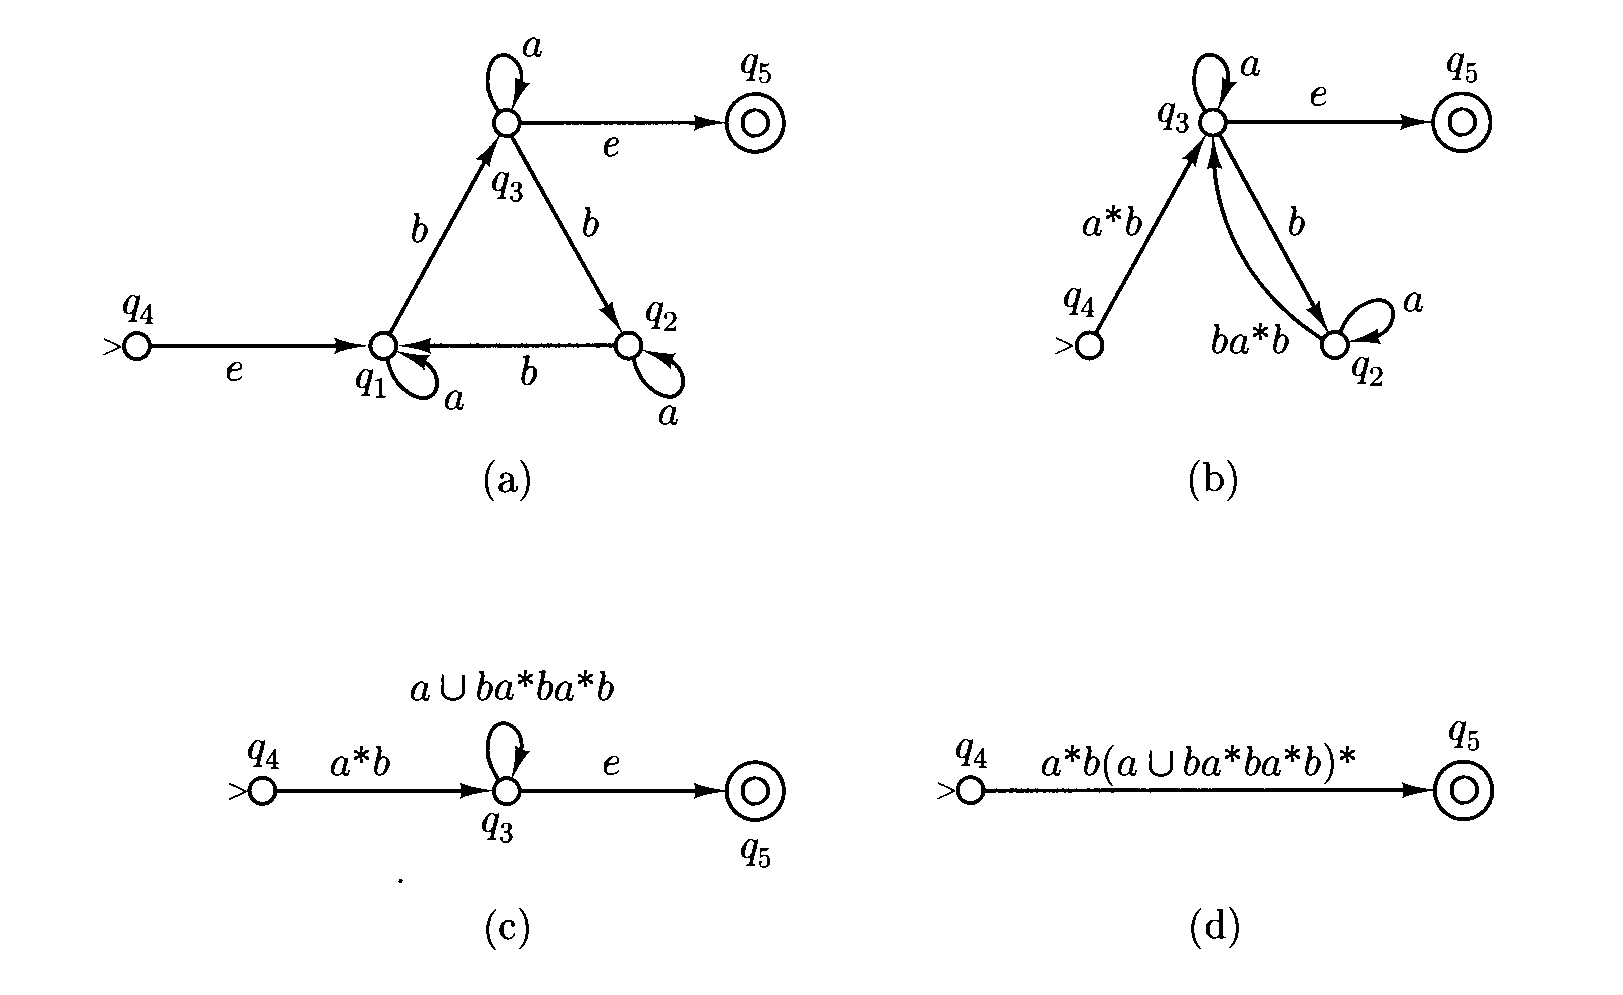
\includegraphics[width=0.6\textwidth]{fa2reg.png}
        \caption{Construct regular expressions from finite automata.}
        \label{fa2reg}
    \end{figure}

    \section{Regular languages}
    \begin{theo}
        (Pumping theorem) Let $L$ be a regular language. 
        \begin{equation}
            \exists n \in \N^* \ \forall w \in L\ \left(|w| \geq n \implies \exists x,y,z \in \Sigma^* \ \forall i \in \N^* \ \begin{cases}
                w = xyz \\ y \neq e \\ |xy| \leq n \\ xy^iz \in L 
            \end{cases}\right)
        \end{equation}
    \end{theo}

    \Proof
    Since $L$ is regular, $L$ is accepted by a DFA $M$. Suppose that $n$ is the number of states of $M$, and let $w$ be a string of length $n$ or greater. 
    
    Consider now the first $n$ steps of the computation of $M$ on $w$:
    \begin{equation*}
        (q_0, w_1 \cdots w_n) \y_M (q_1, w_2 \cdots w_n) \y_M \cdots \y_M (q_n, e)
    \end{equation*}
    By the pigeonhole principle there exist $i$ and $j$, $0 \leq i < j \leq n$, such that $q_i = q_j$. Then the string $y = w_i \cdots w_j$ could be removed from $w$, or repeated any number of times in $w$ just after the $j$-th symbol of $w$, and $M$ would still accept this string. \qed


    \begin{cor}
        \begin{equation}
            \forall n \in \N^* \ \exists w \in L\ |w| \geq n \land \left(
            \begin{cases}
                w = xyz \\ y \neq e \\ |xy| \leq n
            \end{cases}    
            \implies \exists i \geq 0 \ xy^iz \notin L
            \right)
        \end{equation}
        Then $L$ is not a regular.
    \end{cor}

    Applying the theorem correctly can be subtle. It is often useful to think of the application of this result as a game between yourself
    \begin{itemize}
        \item Prover: $L$ is not regular
        \item Adversary: $L$ is regular
    \end{itemize}  
    The theorem states that, once $L$ has been fixed, 
    \begin{enumerate}
        \item the adversary provides a number $n$
        \item you come up with a string $w \in L$ that is longer than $n$
        \item the adversary supplies an appropriate decomposition of $w$ into $xyz$
        \item you point out $i$ for which $xy^iz$ is not in the language.
    \end{enumerate}

    If you have a strategy that always wins, no matter how brilliantly the adversary plays, then you have established that $L$ is not regular.

    \begin{exa}
        \begin{enumerate}
            \item $L = \{ a^ib^i : i \geq 0 \}$ is not regular. $\forall n \in \N^*$, let $w = a^nb^n$, then let $w = xyz$ be a decomposition, then $y = a^i\ (i > 0)$ but $a^{n-i}b^n \notin L$.
            \item $L = \{a^n: n \text{ is prime}\}$ is not regular. Let $w = a^p a^q a^r$ be a decomposition and take $i = (p+2q+r+2)$, then $a^p (a^q)^i a^r = a^{(q+1)(p+2q+r)} \notin L$.
            \item Sometimes it pays to use closure properties to show that a language is not regular.
            \begin{equation}
                L = \{ w \in \{a,b\} : w \text{ has an equal number of a's and b's} \}
            \end{equation}
            $L \cap a^*b^* = \{ a^ib^i : i \geq 0 \}$ is not regular.
        \end{enumerate}
    \end{exa}

    \begin{theo}
        If $L$ is a regular language, then $L^R = \{ w : w^R \in L \}$ is also a regular language.
    \end{theo}
    \Proof
    Consider the automaton $M$ in the special form. Converse the transition relation to get the new automata $M'$ whose start point is the end point of $M'$ and end point is the start point of $M'$.
    \qed

\section{State Minimization}    
    Identifying the reachable states is easy to do in polynomial time, because the set of reachable states can be defined as the closure of $\{s\}$ under the relation $\{(p, q) : a \in \Sigma, \delta(p, a) = q\}$. Therefore, the set of all reachable states can be computed by this simple algorithm:
    \begin{algorithm}[H]
        \caption{Computing reachable states}
        \begin{algorithmic}[1]
            \State $R \l \{ s\}$
            \While{there is a state $p \in R$ and $a \in \Sigma$ such that $\delta(p,a) \notin R$}
            \State $R \l R \cup \{ \delta(p,a) \}$
            \EndWhile
        \end{algorithmic}
    \end{algorithm}

    \begin{defi}
        Two equivalence relations on languages.

        Let $L \subset \Sigma^*$ be a language, and let $x, y \in \Sigma^*$. We say that $x$ and $y$ are equivalent with respect to $L$, denoted $x \approx_L y$, if 
        \begin{equation*}
            \forall z \in \Sigma^* \ (xz \in L \Leftrightarrow yz \in L)
        \end{equation*}

        Let $M = (K, \Sigma, \delta, s, F)$ be a DFA. We say that two strings $x, y \in \Sigma^*$ are equivalent with respect to $M$, denoted $x \sim_M y$, if
        \begin{equation*}
            \exists q \in K \ ((s, x) \ys_M (q, e)) \land ((s, y) \ys_M (q, e))
        \end{equation*}

        Note that $\sim_M$ is less fundamental than $\approx_L$.
    \end{defi}

    \begin{theo}
        Both $\approx_L$ and $\sim_M$ are equivalence relations. The equivalence class of $\sim_M$ can be identified by the states of $M$.
    \end{theo}

    \begin{exa}
        \begin{itemize}
            \item For the regular language $L = \{ \text{the strings that do not contain occurrences of every symbol of the alphabet} \}$, the number of equivalence class is $2^{|\Sigma|}$. Let $A$ and $B$ be two distinct subset of $\Sigma$ and assume that $A$ does not contain $B$. Let $L_X$ be the language consisting of strings which contains every occurrence of symbols of $X$. For $x \in L_A$, $y \in L_B$ and $z \in L_{\Sigma - B}$, $xz \in L$ but $yz \notin L$.
            
            Recall that there is a nondeterministic finite automaton with $|\Sigma| + 1$ states that accepts the same language. Although deterministic automata are exactly as powerful as nondeterministic ones in principle, determinism comes with a price in the number of states which is, at worst, exponential. 
            
            To put it in a different way, and in fact a way that anticipates the important issues of computational complexity: When the number of states is taken into account, \textbf{non-determinism is exponentially more powerful than determinism in the domain of finite automata}.
            \item For the language $L = (ab | ba)^*$, it is not hard to see that $\approx_L$ has four equivalence classes:
            \begin{enumerate}
                \item $[e] = L$
                \item $[a] = La$
                \item $[b] = Lb$
                \item $[aa] = L(aa|bb)\Sigma^*$
            \end{enumerate}
        
            Let $E_q$ denote the equivalence class corresponding to state $q$ of $M$. Then for the automaton in Figure \ref{minimize}
            \begin{figure}[H]
                \centering
                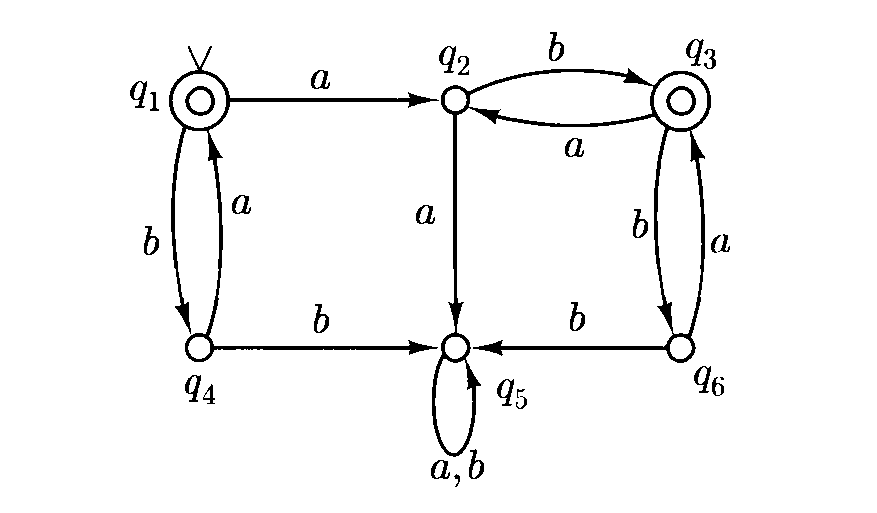
\includegraphics[width=0.5\textwidth]{minimize.png}
                \caption{Minimization}
                \label{minimize}
            \end{figure}
            \begin{enumerate}
                \item $E_{q_1} = (ba)^*$
                \item $E_{q_2} = La$
                \item $E_{q_3} = (ba)^*abL$
                \item $E_{q_4} = b(ab)^*$
                \item $E_{q_5} = L(aa|bb)\Sigma^*$
                \item $E_{q_6} = (ba)^*abLb$
            \end{enumerate}
        \end{itemize}
    \end{exa}

    \begin{defi}
        An equivalence relation $\sim$ is a refinement of another $\approx$ if
        \begin{equation}
            \forall x,y \ x \sim y \implies x \approx y
        \end{equation}
        Each equivalence class of $\approx$ is the union of one or more equivalence classes of $\sim$.
    \end{defi}

    \begin{theo}
        $\sim_M$ is a refinement of $\approx_{L(M)}$, that is
        \begin{equation}
            \forall x,y \in \Sigma^* \ x \sim_M y \implies x \approx_{L(M)} y
        \end{equation}
    \end{theo}

    \begin{theo}
        (The Myhill-Nerode Theorem): Let $L$ be a regular language. Then there is a DFA $M$, $L = L(M)$, and the number of states of $M$ is equal to the number of equivalence classes in $\approx_L$.
    \end{theo}

    \Proof
    Construct the following standard DFA $M$:
    \begin{align*}
        K &= \{ [x] : x \in \Sigma^* \} \\
        s &= [e] \\
        F &= \{ [x] : x \in L \} \\
        \delta([x], a) &= [xa] \ \ \ \ \forall [x] \in K
    \end{align*}

    $L$ is regular $\implies$ $K$ is a finite set. 

    By induction on $|y|$, we have
    \begin{equation}
        ([x], y) \ys_M ([xy], e)
    \end{equation}

    Then
    \begin{align*}
        x \in L(M) 
        &\Leftrightarrow \exists q \in F \ ([e],x) \ys_M (q,e)  \\
        &\Leftrightarrow [x] \in F \\
        &\Leftrightarrow x \in L
    \end{align*}

    Therefore, $L = L(M)$.
    \qed    


    \begin{cor}
        A language $L$ is regular if and only if $L$ has finitely many equivalence classes.
    \end{cor}

    How to compute the standard automaton from a given DFA?

    Define the relation $A_M \subset K \times \Sigma^*$
    \begin{equation*}
        A_M = \{ (q,w) \in K \times \Sigma^*: \exists f \in F \ (q,w) \ys_M (f,e) \}
    \end{equation*}

    Define the equivalence relation $\equiv_n \subset K \times K$
    \begin{equation}
        \equiv_n = \{ (p,q) \in K \times K : \forall z \in \Sigma^* \ (|z| \leq n) \land ((p,z) \in A_M \Leftrightarrow (q,z) \in A_M) \}
    \end{equation}

    Define the equivalence relation $\equiv \subset K \times K$
    \begin{equation}
        \equiv = \{ (p,q) \in K \times K : \forall z \in \Sigma^* \ (p,z) \in A_M \Leftrightarrow (q,z) \in A_M \}
    \end{equation}
    The equivalence classes of $\equiv$ are precisely those sets of states of $M$ that must be clumped together in order to obtain the standard automaton of $L(M)$.

    For the example in Figure \ref{minimize}
    \begin{equation*}
        [e] = E_{q_1} \cup E_{q_3} \ \ \ \ [b] = E_{q_4} \cup E_{q_6}
    \end{equation*}

    \begin{exa}
        The standard automaton corresponding to the language $L = (ab | ba)^*$ is
        \begin{figure}[H]
            \centering
            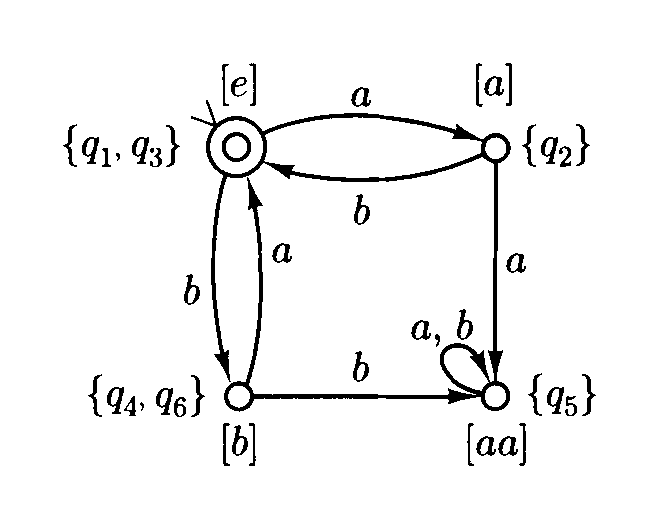
\includegraphics[width=0.4\textwidth]{standard.png}
            \caption{standard automaton}
            \label{standard}
        \end{figure}
    \end{exa}

    We can compute the equivalence classes of $\equiv$ step by step.

    \begin{lemma}
        For any two states $q,p \in K$ and any integer $n \geq 1$
        \begin{equation}
            q \equiv_n p \Longleftrightarrow 
            \begin{cases}
                q \equiv_{n-1} p \\ \forall a \in \Sigma \ \delta(q,a) \equiv_{n-1} \delta(p,a)
            \end{cases}
        \end{equation}
    \end{lemma}

    \begin{algorithm}[H]
        \caption{Computing the standard automata}
        \begin{algorithmic}[1]
            \State Initially the equivalence classes of $\equiv_0$ are $F$ and $K - F$
            \Repeat
            \For {$n = 1,2,\cdots$}
            \State compute the equivalence classes of $\equiv_n$ from those $\equiv_{n-1}$ 
            \EndFor
            \Until $\equiv_n$ is the same as $\equiv_{n-1}$
        \end{algorithmic}
    \end{algorithm}

\section{Context-Free Languages}
    \begin{defi}
        A context-free grammar $G$ is a quadruple $(V, \Sigma, R, S)$, where
        \begin{enumerate}
            \item $V$ is an alphabet
            \item $\Sigma \subset V$ is the set of terminals
            \item $R \subset (V - \Sigma) \times V^*$
            \item $S \in V - \Sigma$ is the start symbol 
        \end{enumerate}
        \begin{itemize}
            \item The members of $V-\Sigma$ are called nonterminals. 
            \item For any $A \in V-\Sigma$ and $u \in V^*$, 
            \begin{equation}
                A \to_G u \Longleftrightarrow (A,u) \in R 
            \end{equation}
            \item For any strings $u, v \in V^*$
            \begin{equation}
                u \Rightarrow_G v \Longleftrightarrow \exists x,y,w \in V^* ,\ A \in V - \Sigma \ \begin{cases}
                    u = xAy \\ v = xwy \\ A \to_G w
                \end{cases}
            \end{equation}
            \item The relation $\Rightarrow_G^*$ is the reflexive, transitive closure of $\Rightarrow_G$.
            \item $L(G)$, the language generated by $G$, is
            \begin{equation}
                L(G) = \{ w \in \Sigma^* : S \Rightarrow_G^* w \}
            \end{equation}
            \item A language $L$ is said to be a context-free language if $L = L(G)$ for some context-free grammar $G$.
        \end{itemize}
    \end{defi}

    \begin{defi}
        We call any sequence of the form
        \begin{equation}
            w_0 \Rightarrow_G w_1 \Rightarrow_G \cdots \Rightarrow_G w_n
        \end{equation}
        an $n$-step derivation in $G$ of $w_n$ from $w_0$.
    \end{defi}

    \begin{exa}
        The following grammar $G = (V, \Sigma, R, S)$ generates the irregular language $\{a^ib^i : i \in \N\}$
        \begin{align*}
            V &= \{ S,a,b \} \\
            \Sigma &= \{a,b\} \\
            R &= \{ S \to aSb, S \to e \}
        \end{align*}
    \end{exa}

    \begin{theo}
        All regular languages are context-free.
    \end{theo}
    \Proof
    Consider the regular language accepted by the deterministic finite
    automaton $M = (K, \Sigma, \delta, s, F)$. The same language is generated by the grammar $G(M) = (V, \Sigma, R, S)$, where $V = K \cup \Sigma$, $S = s$, and $R$ consists of these rules:
    \begin{equation}
        R = \{ q \to ap : \delta(q,a)=p \} \cup \{ q \to e: q \in F \}
    \end{equation}
    \qed

    Let $G$ be a CFG. A string $w \in L(G)$ may have many derivations in $G$. Intuitively, parse trees are ways of representing derivations of strings in $L(G)$ so that the superficial differences between derivations, owing to the order of application of rules, are suppressed. To put it otherwise, parse trees represent equivalence classes of derivations. 
    \begin{defi}
        For a context-free grammar $G = (V, \Sigma, R, S)$, we define its \textbf{parse trees} and their roots, leaves, and yields, as follows.
        \begin{enumerate}
            \item $\forall a \in \Sigma$ is a parse tree. The single node of this parse tree is both the root and a leaf. The yield of this parse tree is a.
            \item If $A \to a$ is a rule, then there is a parse tree whose root is the node labeled $A$, its sole leaf is the node labeled $e$, and its yield is $e$.
            \item Given $n$ parse trees, where $n > 1$, with roots labeled $A_1, \cdots, A_n$ respectively, and with yields $Y_1, \cdots , Y_n$, and $A \to A_1 \cdots A_n$ is a rule in $R$, then we can construct a parse tree. Its root is the new node labeled $A$, its leaves are the leaves of its
            constituent parse trees, and its yield is $Y_1 \cdots Y_n$.
            \item Nothing else is a parse tree.
        \end{enumerate}

        We say that two derivations $D$ and $D'$ are \textbf{similar} if the pair $(D, D')$ belongs in the reflexive, symmetric, transitive closure of $\prec$. 
    \end{defi}

    \begin{defi}
        Let $D,D'$ be derivations in a CFG $G$. $D \prec D'$ iff
        \begin{enumerate}
            \item $x_i = x'_i \ \ \forall i \neq k$
            \item $x_{k-1} = x'_{k-1} = uAvBw$ where $u,v,w \in V^*$ and $A,B \in V-\Sigma$
            \item $x_k = vyvBw$ where $A \to y \in \R$
            \item $x'_k = uAvzw$ where $B \to z \in \R$
            \item $x_{k+1} = x'_{k+1} = uyvzw$
        \end{enumerate}
    \end{defi}

    \begin{theo}
        Let $G = (V,\Sigma,R,S)$ be a CFG, and let $A \in V - \Sigma$, and $w \in \Sigma^*$. Then the following statements are equivalent
        \begin{enumerate}
            \item $A \Rightarrow^* w$
            \item There is a parse tree with root $A$ and yield $w$
            \item $A \Rightarrow_L^* w$
            \item $A \Rightarrow_R^* w$
        \end{enumerate}
    \end{theo}

    \begin{defi}
        Grammars with strings that have two or more distinct parse trees, are called \textbf{ambiguous}. In fact, there are context-free languages with the property that all context-free grammars that generate them must be ambiguous. Such languages are called \textbf{inherently ambiguous}.
    \end{defi}
    

    \section{Pushdown automaton}
    \begin{defi}
        \textbf{Pushdown automaton} is defined to be a sextuple $M = ( K , \Sigma , \Gamma , \Delta, s , F )$ , where
        \begin{enumerate}
            \item $K$ is a finite set of states
            \item $\Sigma$ is an alphabet (the input symbols)
            \item $\Gamma$ is an alphabet (the stack symbols)
            \item $s \in K$ is the initial state
            \item $F \in K$ is the set of final states
            \item $\Delta \subset (K \times (\Sigma \cup \{e\}) \times \Gamma^*) \times (K \times \Gamma^*)$ is a finite transition relation.
        \end{enumerate}
        \begin{itemize}
            \item If $((p, a, \beta), (q, \gamma)) \in \Delta$ then M, whenever it is in state $p$ with $\beta$ at the top of the stack, may read $a$ from the input tape, replace $\beta$ by $\gamma$, on the top of the stack, and enter state $q$. Such a pair $((p, a, \beta), (q, \gamma))$ is called a \textbf{transition} of $M$. To \textbf{push} a symbol is to add it to the top of the stack; to \textbf{pop} a symbol is to remove it from the top of the stack.
            
            \item A \textbf{configuration} of a pushdown automaton is defined to be a member of $K \times \Sigma^* \times \Gamma^*$: The first component is the state of the machine, the second is the
            portion of the input yet to be read, and the third is the contents of the pushdown store, read top-down.

            \item \textbf{Yield} 
            \begin{equation}
                ((p, a, \beta), (q, \gamma)) \in \Delta \Longleftrightarrow (p, ay, \beta\eta) \y_M (q, y, \gamma\eta)
            \end{equation}

            \item We denote the reflexive, transitive closure of $\y_M$ by $\y_M^*$.

            \item A string $w \in \Sigma^*$ is accepted by $M$ iff
            \begin{equation}
                \exists q \in F \ (s, w, e) \y_M^* (q,e,e)
            \end{equation}

            \item The language accepted by $M$, denoted $L(M)$, is the set of all strings accepted by $M$.
        \end{itemize}
    \end{defi}

    \begin{exa}
        The PDA $M = (K,\Sigma,\Gamma,\Delta,s,F)$ to accept the language $L = \{ wcw^R : w \in \{a,b\}^* \}$.
        \begin{align*}
            K &= \{s,f\} \ \ \Sigma = \{a,b,c\} \ \ \Gamma = \{a,b\} \ \ F = \{f\} \\
            \Delta &= \{ \\
                & ((s,a,e),(s,a)), \\
                & ((s,b,e),(s,b)), \\
                & ((s,c,e),(f,e)), \\
                & ((f,a,a),(f,e)), \\
                & ((f,b,b),(f,e)) \\
            \} &
        \end{align*}
    \end{exa}

    \begin{exa}
        The PDA $M = (K,\Sigma,\Gamma,\Delta,s,F)$ to accept the language $L = \{ ww^R : w \in \{a,b\}^* \}$.
        \begin{align*}
            K &= \{s,f\} \ \ \Sigma = \{a,b\} \ \ \Gamma = \{a,b\} \ \ F = \{f\} \\
            \Delta &= \{ \\
                & ((s,a,e),(s,a)), \\
                & ((s,b,e),(s,b)), \\
                & ((s,e,e),(f,e)), \\
                & ((f,a,a),(f,e)), \\
                & ((f,b,b),(f,e)) \\
            \} &
        \end{align*}
    \end{exa}

    \begin{exa}
        The PDA $M = (K,\Sigma,\Gamma,\Delta,s,F)$ to accept the language 
        \begin{equation*}
            L = \{ w \in \{a,b\}^* : \text{w has the same number of a's and b's} \}
        \end{equation*}
        \begin{align*}
            K &= \{s,q,f\} \ \ \Sigma = \{a,b\} \ \ \Gamma = \{a,b,c\} \ \ F = \{f\} \\
            \Delta &= \{ \\
                & ((s,e,e),(q,c)), \\
                & ((q,a,c),(q,ac)), \\
                & ((q,a,a),(q,aa)), \\
                & ((q,a,b),(q,e)), \\
                & ((q,b,c),(q,bc)), \\
                & ((q,b,b),(q,bb)), \\
                & ((q,b,a),(q,e)), \\
                & ((q,e,c),(f,e)) \\
            \} &
        \end{align*}
    \end{exa}

    \begin{theo}
        Every finite automaton can be trivially viewed as a PDA that never operates on its stack.
    \end{theo}
    \Proof
    \begin{equation}
        M = (K, \Sigma, \Delta, s, F)
    \end{equation}
    \begin{equation}
        M' = (K, \Sigma, \emptyset, \Delta', s, F)
    \end{equation}
    where
    \begin{equation}
        \Delta' = \{ ((p,u,e),(q,e)) : (p,u,q) \in \Delta \}
    \end{equation}

    We have $L(M) = L(M')$. \qed

    \begin{defi}
        A PDA $M = (K, \Sigma, \Gamma, \Delta, s, F)$ is simple if
        \begin{equation}
            \begin{cases}
                q \neq s \\
                ((q, a, \beta), (p, \gamma)) \in \Delta
            \end{cases}
            \implies \begin{cases}
                |\beta| = 1 \\
                |\gamma| \leq 2
            \end{cases}
        \end{equation}
    \end{defi}
    \begin{theo}
        If a language is accepted by an unrestricted PDA, then it is accepted by a simple PDA.
    \end{theo}
    \Proof
        Let $M = (K,\Sigma,\Gamma,\Delta,s,F)$ be a PDA. 
        We shall construct a simple PDA $M' = (K', \Sigma, \Gamma \cup \{Z\}, \Delta', s', \{f'\})$ that also accepts $L(M)$, where $K' = K \cup \{ s', f' \}$ and $\Delta'$ consists of
        \begin{enumerate}
            \item start transition: $((s',e,e),(s,Z))$
            \item final transitions: $\forall f \in F, \ ((f,e,Z),(f',e))$
            \item the transitions transformed from those in $\Delta$
        \end{enumerate}
    \qed

    \begin{theo}
        Each context-free language is accepted by some PDA. 
    \end{theo}
    \Proof
    Let $G = (V, \Sigma, R, S)$ be a context-free grammar; we must construct a PDA $M$ such that $L(M) = L(G)$. The machine we construct has only two states, $p$ and $q$, and remains permanently in state $q$ after its first move. Also, $M$ uses $V$, the set of terminals and nonterminals, as its stack alphabet. We let
    \begin{equation}
        M = (\{p,q\}, \Sigma, V, \Delta, p, \{q\})
    \end{equation}
    where $\Delta$ contains the following transitions:
    \begin{enumerate}
        \item $((p,e,e),(q,S))$
        \item $((q,e,A),(q,x))$ for each rule $A \to x$ in $R$
        \item $((q,a,a),(q,e))$ for each $a \in \Sigma$
    \end{enumerate}

    % The PDA $M$ begins by pushing $S$, the start symbol of $G$, on its initially empty pushdown store, and entering state $q$ (transition 1). On each subsequent step, it either replaces the topmost symbol $A$ on the stack, provided that it is a nonterminal, by the right-hand side $x$ of some rule $A \to x$ in $R$ (transitions of type 2), or pops the topmost symbol from the stack, provided that it is a terminal symbol that matches the next input symbol (transitions of
    % type 3). The transitions of $M$ are designed so that the pushdown store during an accepting computation mimics a leftmost derivation of the input string; $M$ intermittently carries out a step of such a derivation on the stack, and between such steps it strips away from the top of the stack any terminal symbols and matches them against symbols in the input string. Popping the terminals from the stack has in turn the effect of exposing the leftmost nonterminal, so that the process can continue.

    To continue the proof, in order to establish that $L(M) = L(G)$, we prove the following claim: Let $w \in \Sigma^*$ and $\alpha \in (V-\Sigma)V^* \cup \{ e \}$. Then
    \begin{equation}
        S \xRightarrow{L}^* w\alpha \Longleftrightarrow (q,w,S) \ys_M (q,e,\alpha)
    \end{equation}
    Taking $\alpha = e$ completes the proof.

    The following is proof of the claim.
    \begin{enumerate}
        \item To prove $S \xRightarrow{L}^* w\alpha \implies (q,w,S) \ys_M (q,e,\alpha)$, induction on the number of derivations.
        
        Basis Step. If the derivation is of length 0. then $w = e, \alpha = S$ and hence $(q,w,S) \ys_M (q,e,\alpha)$.
        
        Induction Hypothesis. Suppose $S \xRightarrow{L}^* w\alpha \implies (q,w,S) \ys_M (q,e,\alpha)$ holds when the derivation is of length $n$ or less.

        Induction Step. Consider the derivation of length $n+1$:
        \begin{equation}
            S = u_0 \Rightarrow \cdots \Rightarrow u_n \Rightarrow u_{n+1} = w\alpha
        \end{equation} 
        Let $u_n = xA\beta$, then
        \begin{equation}
            (q,x,S) \ys_M (q, e, A\beta)
        \end{equation}

        Suppose the $(n+1)$-th derivation use the rule $A \to \gamma$, then
        \begin{equation}
            x\gamma\beta = w\alpha = xy\alpha
        \end{equation}
        \begin{equation}
            (q,w,S) = (q,xy,S) \ys_M (q,y,A\beta) \y_M (q,y,\gamma\beta) \y_M^* (q,e,\alpha)
        \end{equation}

        \item To prove $(q,w,S) \ys_M (q,e,\alpha) \implies S \xRightarrow{L}^* w\alpha$, induction on the number of type 2 transitions.
        
        Basis Step: if there are no type-2-transtion, then $w = e$ and $\alpha = S$, thus $S \xRightarrow{L}^* w\alpha = S$.

        Induction Hypothesis. Suppose $(q,w,S) \ys_M (q,e,\alpha) \implies S \xRightarrow{L}^* w\alpha$ holds when there are no more that $n$ type-2-transtions.

        Induction Step. Consider the computation with $n+1$ type 2 transitions. The last type-2-transtion is operated on $(q, y, A\beta)$ and the rule is $A \to \gamma$. 
        \begin{equation}
            (q,w,S) \ys_M (q,y,A\beta) \y_M (q,y,\gamma\beta) \ys_M (q,e,\alpha)
        \end{equation}
        \begin{equation}
            \gamma\beta = y\alpha
        \end{equation}
        According to induction hypothesis
        \begin{equation}
            S \xRightarrow{L}^* xA\beta \xRightarrow{L}^* x\gamma\beta = xy\alpha = w\alpha
        \end{equation}
    \end{enumerate}
    \qed

    \begin{theo}
        If a language is accepted by a PDA, it is a context-free language.
    \end{theo}
    \Proof
    Let $M = (K,\Sigma,\Gamma,\Delta,s,F)$ be a PDA. 
    There is a simple PDA $M' = (K', \Sigma, \Gamma \cup \{Z\}, \Delta', s', \{f'\})$ that also accepts $L(M)$, where $K' = K \cup \{ s', f' \}$. Let $G = (V,\Sigma,R,S)$ where $V$ consists of
    \begin{enumerate}
        \item $S$ and each symbol in $\Sigma$
        \item $\< q,A,p \> \ \ \ \ q,p \in K' \ A \in \Gamma \cup \{ e,Z \}$
    \end{enumerate}
    \qed

    % \begin{exa}
    %     The PDA $M = (K,\Sigma,\Gamma,\Delta,s,F)$ to accept the language $L = \{ wcw^R : w \in \{a,b\}^* \}$.
    %     \begin{align*}
    %         K &= \{s,f\} \ \ \Sigma = \{a,b,c\} \ \ \Gamma = \{a,b\} \ \ F = \{f\} \\
    %         \Delta &= \{ \\
    %             & ((s,a,e),(s,a)), \\
    %             & ((s,b,e),(s,b)), \\
    %             & ((s,c,e),(f,e)), \\
    %             & ((f,a,a),(f,e)), \\
    %             & ((f,b,b),(f,e)) \\
    %         \} &
    %     \end{align*}
    %     Convert it to a context-free language.
    % \end{exa}
    % Let $M' = (K', \Sigma, \Gamma \cup \{ Z \}, \Delta', s', \{ f' \})$ where $K' = \{s,f,s',f'\}$ and
    % \begin{align*}
    %     \Delta' &= \{ \\
    %             & ((s',e,e),(s,Z)), \\
    %             & ((s,a,a),(s,aa)), \\
    %             & ((s,a,b),(s,ab)), \\
    %             & ((s,a,Z),(s,aZ)), \\
    %             & ((s,b,a),(s,ba)), \\
    %             & ((s,b,b),(s,bb)), \\
    %             & ((s,b,Z),(s,bZ)), \\
    %             & ((s,c,a),(f,a)), \\
    %             & ((s,c,b),(f,b)), \\
    %             & ((s,c,Z),(f,Z)), \\
    %             & ((f,a,a),(f,e)), \\
    %             & ((f,b,b),(f,e)) \\
    %             & ((f,e,Z),(f',e)) \\ 
    %         \}
    % \end{align*}

    % Construct the grammar $G = (V,\Sigma,R,S)$
    % \begin{equation*}
    %     V = \{ S, a,b,c \} \cup \{ \< q,A,p \> : q,p \in K', A \in \Gamma \cup \{ e,Z \} \}
    % \end{equation*}
    % The rules in $R$ are of four types.
    % \begin{enumerate}
    %     \item $S \to \< s,Z,f' \>$
    %     \item Let $p \in K'$
    %     \begin{align*}
    %         &\< s,a,p \> \to c \< f,a,p \> \\
    %         &\< s,b,p \> \to c \< f,b,p \> \\
    %         &\< s,Z,p \> \to c \< f,Z,p \> \\
    %         &\< f,a,p \> \to a \< f,e,p \> \\
    %         &\< f,b,p \> \to b \< f,e,p \> \\
    %         &\< f,Z,p \> \to \< f',e,p \> \\
    %     \end{align*}
    %     \item Let $p,p' \in K'$
    %     \begin{align*}
    %         &\< s,a,p \> \to a \< s,a,p' \> \< p',a,p \> \\
    %         &\< s,b,p \> \to a \< s,a,p' \> \< p',b,p \> \\
    %         &\< s,Z,p \> \to a \< s,a,p' \> \< p',Z,p \> \\
    %         &\< s,a,p \> \to b \< s,b,p' \> \< p',a,p \> \\
    %         &\< s,b,p \> \to b \< s,b,p' \> \< p',b,p \> \\
    %         &\< s,Z,p \> \to b \< s,b,p' \> \< p',Z,p \> \\
    %     \end{align*}

    %     \item $p \in K', \ \<p,e,p\> \to e$
    % \end{enumerate}

    \begin{theo}
        The context-free languages are closed under union, concatenation, and Kleene star.
    \end{theo}

    \begin{theo}
        The intersection of a context-free language with a regular language is a context-free language.
    \end{theo}

    \section{Turing Machines}
    \begin{defi}
        A Turing machine is a quintuple $(K, \Sigma, \delta, s, H)$, where
        \begin{enumerate}
            \item $K$ is a finite set of states
            \item $\Sigma$ is an alphabet such that $\{ \sqcup, \rhd \} \subset \Sigma$ and $\{\leftarrow, \rightarrow\} \not\subset \Sigma$.
            \item $s \in K$ is the initial state
            \item $H \subset K$ is the set of halting states
            \item $\delta : (K-H) \times \Sigma \to K \times (\Sigma \cup \{ \leftarrow, \rightarrow \})$ is the transition function which satisfies
            \begin{enumerate}
                \item $\forall q \in K-H, \ \delta(q,\rhd) = (p, \rightarrow)$ for some $p \in K$
                \item $\forall q \in K-H$, $p \in K$ and $a \in \Sigma, \ \delta(q,a) \neq (p, \rhd)$
            \end{enumerate}
        \end{enumerate}
    \end{defi}

    \begin{defi}
        A configuration of a Turing machine $M = (K, \Sigma, \delta, s, H)$ is a member of $K \times \rhd \Sigma^* \times ( \Sigma^* (\Sigma - \{ \sqcup \}) \cup \{ e \} )$.
    \end{defi}

    \begin{exa}
        Consider the Turing machine $M = (K, \Sigma, \delta, s, \{h\})$ where 
        \begin{align*}
            K &= \{ q_0, q_1, h \} \\
            \Sigma &= \{ a, \sqcup, \rhd \} \\
            s &= q_0
        \end{align*}
        The transition function $\delta$ is defined as
        \begin{align*}
            \delta(q_0, a)      &= (q_1, \sqcup) \\
            \delta(q_0, \sqcup) &= (h, \sqcup) \\
            \delta(q_0, \rhd)   &= (q_0, \rightarrow) \\
            \delta(q_1, a)      &= (q_0, a) \\
            \delta(q_1, \sqcup) &= (q_0, \rightarrow) \\
            \delta(q_1, \rhd)   &= (q_1, \rightarrow)
        \end{align*}

        When $M$ is started in its initial state $q_0$, it scans its head to the right, changing all $a$'s to $\sqcup$'s as it goes, until it finds a tape square already containing $\sqcup$; then it halts. 
    \end{exa}

    \begin{exa}
        Basic Turing machines:
        \begin{enumerate}
            \item Move left: $L = (\{s,h\}, \Sigma, \delta, s, \{h\})$, $\delta(s, \sigma) = \begin{cases}
                (h, \l) & \sigma \in \Sigma - \{ \rhd \} \\
                (s, \r) & \sigma = \rhd \\
            \end{cases}$
            \item Move right: $R = (\{s,h\}, \Sigma, \delta, s, \{h\})$, $\delta(s, \sigma) = \begin{cases}
                (h, \r) & \sigma \in \Sigma - \{ \rhd \} \\
                (s, \r) & \sigma = \rhd \\
            \end{cases}$
            \item Write: $M_a = (\{s,h\}, \Sigma, \delta, s, \{h\})$, $\delta(s, b) = \begin{cases}
                (h, a) & b \in \Sigma - \{ \rhd \} \\
                (s, \r) & b = \rhd
            \end{cases}$
        \end{enumerate}
    \end{exa}

    \begin{defi}
        The Rules for Combining Machines. Turing machines will be combined in a way suggestive of the structure of a finite automaton. Individual machines are like the states of a finite automaton, and the machines may be connected to each other in the way that the states of a finite automaton are connected together. However, the connection from one machine to another is not pursued until the first machine halts; the other machine is then started from its initial state with the tape and head position as they were left by the first machine. So if $M_1$ , $M_2$ and $M_3$ are Turing machines, the machine operates as follows: Start in the initial state of $M_1$; operate as $M_1$ would operate until $M_1$ would halt; then, if the currently scanned symbol is an $a$, initiate $M_2$ and operate as $M_2$ would operate; otherwise, if the currently scanned symbol is a $b$, then initiate $M_3$ and operate as $M_3$ would operate.

        A formal definition is
        \begin{align*}
            K &= K_1 \cup K_2 \cup K_3 \\
            s &= s_1 \\
            H &= H_2 \cup H_3 \\
            \delta(q, \sigma) &= \begin{cases}
                \delta_1(q, \sigma) & q \in K_1 - H_1 \\
                \delta_2(q, \sigma) & q \in K_2 - H_2 \\
                \delta_3(q, \sigma) & q \in K_3 - H_3 \\
                (s_2, \sigma) & q \in H_1,\ \sigma=a \\
                (s_3, \sigma) & q \in H_1,\ \sigma=b \\
                (h, \sigma) & h \in H,\ \sigma \neq a,b
            \end{cases}
        \end{align*}
    \end{defi}

    \begin{defi}
        Let $M = (K, \Sigma, \delta, s, \{y,n\})$ be a TM.
        \begin{itemize}
            \item accepting configuration: the halting configuration whose state component is $y$ 
            \item rejecting configuration: the halting configuration whose state component is $n$ 
            \item $M$ accepts $w \in (\Sigma-\{ \sqcup,\rhd \})^*$ if $(s, \rhd \u \sqcup w)$ yields an accepting configuration
            \item $M$ rejects $w \in (\Sigma-\{ \sqcup,\rhd \})^*$ if $(s, \rhd \u \sqcup w)$ yields an rejecting configuration
        \end{itemize}

        Let $\Sigma_0 \subset \Sigma - \{ \sqcup, \rhd \}$ be the input alphabet. We say that $M$ decides a language $L \subset \Sigma_0^*$ if
        \begin{equation*}
            \begin{cases}
                w \in L \implies $M$ \text{ accepts } $w$ \\
                w \notin L \implies $M$ \text{ rejects } $w$
            \end{cases}
        \end{equation*}

        A language $L$ is \textbf{recursive} if there is a Turing machine that decides it.
    \end{defi}

    \begin{rem}
        There is a subtle point in relation to Turing machines that decide languages: With the other language recognizers that we have seen so far in this book (even the nondeterministic ones), one of two things could happen: either the machine accepts the input, or it rejects it. A Turing machine, on the other hand, even if it has only two halt states $y$ and $n$, always has the option of evading an answer (``yes'' or ``no''), by \textbf{failing to halt}. Given a Turing machine, it might or it might not decide a language -- and there is no obvious way to tell whether it does. The far-reaching importance -- and necessity -- of this deficiency will become apparent later in this chapter and in the next.
    \end{rem}

    \begin{defi}
        Let $M = (K, \Sigma, \delta, s, \{h\})$ be a TM. Suppose
        \begin{equation*}
            (s, \rhd \u \sqcup x) \ys_M (h, \rhd \u \sqcup y) 
        \end{equation*}
        where $x,y \in \Sigma_0^*$ and $\Sigma_0 \subset \Sigma - \{ \sqcup, \rhd \}$ is the input alphabet.

        Then $y$ is called the output of $M$ on input $x$, and is denoted $M(x)$. Notice that $M(x)$ is defined only if $M$ halts on input $x$.

        Let $f: \Sigma_0^* \to \Sigma_0^*$. We say that $M$ computes function $f$ if 
        \begin{equation*}
            M(x) = f(x) \ \ \ \ \forall x \in \Sigma_0^*
        \end{equation*}

        A function $f$ is called \textbf{recursive}, if there is a Turing machine $M$ that computes $f$.
    \end{defi}

    \begin{defi}
        Let $M = (K, \Sigma, \delta, s, H)$ be a Turing machine, let $\Sigma_0 \subset \Sigma - \{ \sqcup, \rhd \}$ be an alphabet, and let $L \subset \Sigma_0^*$ be a language. $M$ semidecides $L$ if
        \begin{equation*}
            w \in L \Longleftrightarrow M \text{ halts on } w
        \end{equation*}

        A language $L$ is \textbf{recursively enumerable} if and only if there is a Turing machine $M$ that semidecides $L$.
    \end{defi}

    \begin{theo}
        If a language is recursive, then it is recursively enumerable.
    \end{theo}

    \begin{theo}
        If $L$ is a recursive language, then its complement $\overline L$ is also recursive.
    \end{theo}

    \begin{defi}
        Extentions of Turing machines
        \begin{enumerate}
            \item $k$-tape Turing machine: the transition function is from $(K-H) \times \Sigma^k$ to $K \times (\Sigma \cup \{ \l, \r \})^k$
            \item Two-way Infinite Tape
            \item Multiple Heads
            \item Two-Dimensional Tape
        \end{enumerate}
    \end{defi}

    \begin{theo}
        Any language decided or semidecided, and any function computed by Turing machines with several tapes, heads, two-way infinite tapes, or multi-dimensional tapes, can be decided, semidecided, or computed, respectively, by a standard Turing machine.
    \end{theo}

    \begin{defi}
        A random access Turing machine is a pair $M = (k, \Pi)$ where $k > 0$ is the number of registers, and $\Pi = (\pi_1, \pi2, \cdots ,\pi_p)$, the program, is a finite sequence of instructions. We assume that the last instruction, $\pi_p$, is always a halt instruction (the program may contain other halt instructions as well).

        A configuration of a random access Turing machine $(k, \Pi)$ is a $(k+2)$-tuple $(\kappa, R_0, R_1, \cdots, R_{k-1}, T)$, where $\kappa$ is the program counter. The configuration is called a halted configuration is $\kappa = 0$.

        $T$, the tape contents, is a finite set of pairs of positive integers -- that is, a finite subset of $(\N - \{ 0 \}) \times \{ \N - \{ 0 \} \}$ -- such that $\forall i \geq 1$ there is at most one pair of the form $(i,m) \in T$.
    \end{defi}

    \begin{theo}
        Any language decided or semidecided by a random access Turing machine, and any function computable by a random access Turing machine, can be decided, semidecided, and computed, respectively, by a standard Turing machine. Furthermore, if the machines halt on an input, then the number of steps taken by the standard Turing machine is bounded by a polynomial in the number of steps of the random access Turing machine on the same input.
    \end{theo}

    \section{Grammer}

    \begin{exa}
        The grammar that generates the language $\{ ww : w \in \{ a,b \} \}$
    \end{exa}

    \section{Numerical Functions}

    \section{Undecidability}
    \subsection{the Church-Turing thesis}
    Our notion of an algorithm must exclude Turing machines that may not halt on some inputs. We therefore propose to adopt the Turing machine that halts on all inputs as the precise formal notion corresponding to the intuitive notion of an ``algorithm''. Nothing will be considered an algorithm if it cannot be rendered as a Turing machine that is guaranteed to halt on all inputs, and all such machines will be rightfully called algorithms. This principle is known as the \textbf{Church-Turing thesis}. It is a thesis, not a theorem, because it is not a mathematical result: It simply asserts that a certain informal concept (algorithm) corresponds to a certain mathematical object (Turing machine). Not being a mathematical statement, the Church-Turing thesis cannot be proved. It is theoretically possible, however, that the Church-Turing thesis could be disproved at some future date, if someone were to propose an alternative model of computation that was publicly acceptable as a plausible and reasonable model of computation, and yet was provably capable of carrying out computations that cannot be carried out by any Turing machine. No one considers this likely. 
    
    Adopting a precise mathematical notion of an algorithm opens up the intriguing possibility of formally proving that certain computational problems cannot be solved by any algorithm. We already know enough to expect this. In Chapter 1 we argued that if strings are used to represent languages, not every language can be represented: there are only a countable number of strings over an alphabet, and there are uncountably many languages. Finite automata, pushdown automata, context-free grammars, unrestricted grammars, and Turing machines are all examples of finite objects that can be used for specifying languages, and that can be themselves described by strings (in the next section we develop in detail a particular way of representing Turing machines as strings). Accordingly, there are only countably many recursive and recursively enumerable languages over any alphabet. So although we have worked hard to extend the capabilities of computing machines as far as possible, in absolute terms they can be used for semideciding or deciding only an infinitesimal fraction of all the possible languages. 
    
    Using cardinality arguments to establish the limitation of our approach is trivial; finding particular examples of computational tasks that cannot be accomplished within a model is much more interesting and rewarding. In earlier chapters we did succeed in finding certain languages that are not regular or context-free; in this chapter we do the same for the recursive languages. There are two major differences, however. 
    \begin{enumerate}
        \item First, these new negative results are not just temporary setbacks, to be remedied in a later chapter where an even more powerful computational device will be defined: according to the Church-Turing thesis, computational tasks that cannot be performed by Turing machines are impossible, hopeless, undecidable. 
        \item Second, our methods for proving that languages are not recursive will have to be different from the "pumping" theorems we used for exploiting the weaknesses of context-free grammars and finite au-tomata. Rather, we must devise techniques for exploiting the considerable power of Turing machines in order to expose their limitations.
    \end{enumerate}

    \subsection{The halting problem}

    The Turing machine (program) $\mathsf{halts}$ is defined as the Turing machine that takes $P$, an arbitrary Turing machine (program), and $X$, the input of $P$, as input, and decides whether $P$ halts with input $X$.

    \begin{theo}
        $\mathsf{halts}$ does not exists.
    \end{theo}
    \Proof
    Suppose $\mathsf{halts}$, define the following program:
    \begin{lstlisting}
        diag(X):
            if halts(X, X) then
                loop infinitely
            else
                halt
    \end{lstlisting}

    Then consider the process diag(diag):
    \begin{align*}
        &\text{diag(diag) halts} \Longleftrightarrow \text{halts(diag, diag)} \implies  \text{diag(diag) does not halt} \\
        &\text{diag(diag) does not halt} \Longleftrightarrow \text{!halts(diag, diag)} \implies \text{diag(diag) halts}
    \end{align*}
    This comes to a contradiction. Hence there must not be a $\mathsf{halts}$ program. \qed

    \begin{theo}
        (Rice's Theorem): Suppose that $\mathcal C$ is a proper, nonempty subset of the class of all recursively enumerable languages. Then the following problem is undecidable: Given a Turing machine $M$, is $L(M) \in \mathcal C$?    
    \end{theo}

    We can assume that $\emptyset \in \mathcal C$ and $L \in \mathcal C$. We can construct $T_M$ such that the language semidecided by $T_M$ is either the language $L$ or $\emptyset$.

    Let $M_L$ be a TM that semidecides $L$. $T_M$ first simulate UTM on input ``$M$''. If $M$ halts on $e$, then $T_M$ goes on to simulate the $M_L$ on input $x$, if it halts, then accept. Otherwise, $T_M$ rejects input $x$.

    It is easy to see that $L(T_M) \in \mathcal C$ iff $M$ halts on input $e$. Thus we reduce $H_e$ to the problem. \qed
    
\end{document}